\chapter{Asking Scottsdale Millionaires How They Got Rich}

There is no blackboard in this lecture, and that is worth saying at the outset. The mathematics appears instead in the operator's language of timing, margin, scale, leverage, and choice. What the School of Hard Knocks episode gives us, and what LazyingArt LLC has preserved for us, is a sequence of field examples in which wealth is not a static pile of assets but a moving structure: money comes in, obligations come due, buying power changes with scale, time is reallocated, and compounding appears first as a metaphor and then as a real household mechanism.

\section{Cold Open, Scottsdale, and the Promise of Mechanism}

The lecture begins by stating conclusions before it has earned them. We are shown large business claims, a revenue--profit distinction, and a compounding image. This is not yet argument. It is a promise about the kind of argument to come. The teaser tells us what objects will matter, and only afterward does the speaker restart the discussion on the ground in Scottsdale.

The two quantitative promises that dominate the cold open are a growth ladder and a compounding rule. It is useful to write them in a cleaned form:
\begin{align}
(R_{\text{last}},R_{\text{goal}},R_{+4y})
&=
(160\,\text{M},\,250\,\text{M},\,1\,\text{B}),\\
a_{n+1} &= 2a_n,\qquad a_1 = 0.01,\\
a_n &= 0.01 \cdot 2^{n-1}.
\end{align}

The first line is a ladder of claims and targets, not a forecast derived on the spot. The second and third lines formalize the lecture's ``penny doubled every day'' image. We should keep the recurrence because it captures the pedagogical point: the interesting feature is not the penny, but the update rule. Growth is slow until it is not slow.

The lecture does not pause to settle the indexing ambiguity of the penny example, and we need not force that here. What matters is the narrative function. The host says, in effect, ``you ask how that can happen; here is the compounding picture.'' Only then does the video reset and tell us what we are about to do: travel through Scottsdale, question wealthy operators, and extract the mechanisms rather than merely admire the symbols.

That reset is crucial. The teaser is foreshadowing. The Scottsdale setup is the real beginning.

\section{Revenue, Profit, and the Cash-Poor Paradox}

The first substantive movement begins by attacking a very common confusion. We are told that an entrepreneur can be ``making tens of millions'' and still be dangerously short of cash. The lecture's order matters here. Before it offers a blueprint, it punctures the fantasy that large revenue automatically produces ease.

\begin{definition}
Let \(C_{\text{due}}\) denote the obligations due essentially at once, let \(B\) be the cash balance on hand, and let
\begin{equation}
L_{\text{gap}} = C_{\text{due}} - B
\end{equation}
be the immediate liquidity gap.
\end{definition}

\subsection{Question \& Answer}

\paragraph{Question.} How can someone who is doing large business still be nearly out of cash?

\paragraph{Answer.} Because revenue, profit, and liquidity are different quantities, and they live on different clocks.

The story gives us a worked arithmetic example. An Amex bill of roughly \(550{,}000\) is due the next day, payroll is due the next day as well, and cash in the account is only about \(300{,}000\). Taking payroll in the conservative spirit of the transcript as roughly \(200{,}000\), we obtain
\begin{align}
C_{\text{due}} &\approx 550{,}000 + 200{,}000 = 750{,}000,\\
B &\approx 300{,}000,\\
L_{\text{gap}} &\approx 750{,}000 - 300{,}000 = 450{,}000.
\end{align}

This is the first real derivation in the lecture, even if it is spoken rather than written. The entrepreneur's panic is not psychological excess. It is arithmetic. We are meant to feel the pressure of next-day timing.

The lecture then poses its own practical reply. ``Sales cures everything'' is the compressed slogan, but the mechanism is more precise than the slogan:
\begin{enumerate}
\item ask for time from the creditor;
\item rally the team;
\item assemble a new offer;
\item launch it immediately;
\item convert persuasion into cash before the obligations harden into failure.
\end{enumerate}

The reported result is
\begin{equation}
S_{\text{new}} \approx 800{,}000 > L_{\text{gap}}.
\end{equation}

This is the lecture's first major lesson. Sales is not merely a path to income. Under pressure it becomes a liquidity technology. The host begins here because he wants us to abandon the childish equation
\[
\text{big headline revenue} = \text{financial ease}.
\]
The interview insists that the correct question is always: what cash arrives, in what amount, and by when?

\section{From Sales as Rescue to Leverage: Real Estate, Bigger Deals, and Team Design}

Once the immediate crisis has been resolved, the lecture widens the frame. This is a characteristic move throughout the episode: a local problem is posed, answered concretely, and then generalized. Having shown that sales can close a dangerous gap, the speaker now turns sales into the first member of a broader wealth architecture.

The next recommendation is real estate, in particular what the interview calls the single-tenant triple-net lease game. The idea is not ornament. It is structure.

\begin{definition}
In the lecture's usage, the single-tenant triple-net lease game means owning a property whose tenant is a single strong occupant and whose operating burdens are shifted largely onto that occupant. The examples given are ordinary and institutional: a CVS, a Walgreens, or a doctor's office.
\end{definition}

That recommendation is followed immediately by a second correction. The speaker says that bigger commercial deals may actually be easier than smaller ones. The reason offered is procedural rather than mystical: large institutional deals often collapse into qualification and checklist, whereas smaller deals are more exposed to improvisation, weaker financing, and local friction.

We can summarize the widening structure of the lecture in the following order:
\begin{itemize}
\item sales gives mobility and rescue power;
\item property ownership gives durable claim on income;
\item institutional scale can simplify execution rather than complicate it;
\item the founder must stop being the sole engine if the business is to cross into eight figures.
\end{itemize}

The line ``I fired myself'' is therefore not theater. It is an organizational theorem stated informally: if the firm remains hostage to the founder's personal throughput, it does not truly scale. ``Money loves speed'' follows naturally from this. Speed is not just impatience. It is what happens when competent people, clear roles, and a known checklist replace founder bottleneck.

\section{Blue-Collar Scale: Margin, Purchasing Power, and Bought-Back Time}

The next interview changes the evidentiary tone of the lecture. We leave the war story of cash stress and move to a blue-collar operating system: garage doors, parts, efficiency, and buying power. The point is to show that very large business need not look glamorous in order to be mathematically serious.

The speaker repeats the revenue--profit distinction and gives a large annual revenue claim. That invites the standard identity
\begin{equation}
\Pi = R\,m,
\end{equation}
where \(R\) is revenue, \(\Pi\) is profit, and \(m\) is margin written as a fraction.

The interview's numerical claim is roughly \(R \approx 240\,\text{M}\), together with the statement that the business is ``over \(20\%\) of the bottom line.'' If we interpret that cautiously as a margin claim, then
\begin{equation}
R \approx 240\,\text{M},\qquad m > 0.20
\quad \Longrightarrow \quad
\Pi > 48\,\text{M}.
\end{equation}

\begin{remark}
The phrase ``over \(20\%\) of the bottom line'' is colloquial and ambiguous. We use the inequality only as a standard reconstruction of the lecture's margin logic, not as an audited accounting statement.
\end{remark}

The next piece is scale purchasing. Because the company buys so many doors and parts, it pays less than a smaller firm would pay. The lecture gives the mechanism without the schedule, so we preserve only the qualitative direction:
\begin{equation}
q_2 > q_1
\quad \Longrightarrow \quad
c_{\text{unit}}(q_2) < c_{\text{unit}}(q_1).
\end{equation}

This is enough. The lecture wants us to see that size changes the firm's own input prices. Scale is not only more volume on the revenue side; it can also change the cost function.

From there the interview moves to time. Dan Martell's phrase ``buy back your time'' is used to reframe growth as reallocation rather than mere effort. If \(T_{\text{freed}}\) denotes hours recovered from low-value work, then the lecture's idea can be written as
\begin{equation}
T_{\text{available}}' = T_{\text{available}} + T_{\text{freed}},
\qquad
T_{\text{freed}} \approx 30\ \text{hr/week}.
\end{equation}

We should read this with care. No extra hours are created in a literal week. What changes is deployable capacity. Founder hours are shifted toward work that compounds through systems, judgment, and coordination.

Only after those operational mechanisms are in place does the lecture broaden into a social taxonomy. Millionaires are associated with habits: early rising, cold plunges, church, family discipline. Billionaires are associated with something else: networks, judgment, and the willingness to pay for the best without cheap bargaining. Then the interview narrows again into a three-part attention rule:
\begin{enumerate}
\item focus on what one has rather than obsess only over what one lacks;
\item focus on today and the future rather than on the past;
\item focus on what one can control rather than on what one cannot.
\end{enumerate}

This is not formal mathematics, but it is organized like one of the lecture's control problems. Attention is treated as a limited variable, and wasted attention is treated as genuine drag on performance.

\section{Family Capital Formation as a Small-Scale Compounding Mechanism}

At first glance the sponsor segment looks like a detour. In fact it is structurally aligned with the rest of the lecture. The video has just discussed buying power, efficiency, and compounding at business scale; it now translates that logic into household capital formation. The scale changes. The form of reasoning does not.

\begin{figure}[h]
\centering

\includegraphics[width=0.92\textwidth]{lecture_76_figure_02.png}
\caption{Fabric by Gerber Life gift-card mockup used to illustrate birthday contributions into a child investment flow. The screenshot's evidentiary value lies in the visible interface: ``fabric by Gerber Life,'' ``Charlie,'' ``Grandma \& grandpa,'' \(\text{\$}25\), and ``SEND GIFT.''}
\end{figure}

The frame is worth preserving because it gives the lecture a concrete contribution example. The visible gift amount is
\begin{equation}
G = \text{\$}25.
\end{equation}

The spoken mechanism is that recurring contributions into a child's account can grow over time and later be used for education, extracurricular activity, a first home, or the start of a business. The standard financial reconstruction is
\begin{equation}
FV = \sum_{k=0}^{n-1} c(1+r)^k,
\end{equation}
where \(c\) is the recurring contribution and \(r\) is the per-period growth rate.

The transcript also mentions a contribution as small as \(\text{\$}1\) a day, but that figure is not visible in the screenshot. The screenshot gives us the concrete, frame-backed example \(G=\text{\$}25\); the recurrence formula gives us the general compounding mechanism.

A small schematic may help isolate the logic while keeping the screenshot as the primary evidence:
\begin{figure}[h]
\centering
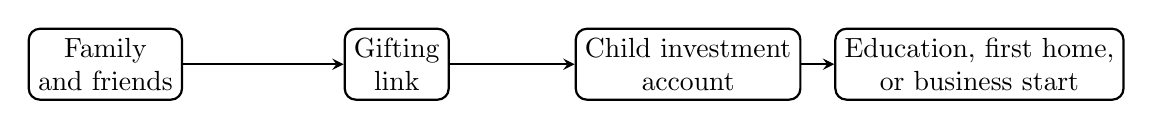
\begin{tikzpicture}[>=stealth, thick]
\node[draw, rounded corners, align=center] (a) at (0,0) {Family\\and friends};
\node[draw, rounded corners, align=center] (b) at (3.7,0) {Gifting\\link};
\node[draw, rounded corners, align=center] (c) at (7.4,0) {Child investment\\account};
\node[draw, rounded corners, align=center] (d) at (11.1,0) {Education, first home,\\or business start};
\draw[->] (a) -- (b);
\draw[->] (b) -- (c);
\draw[->] (c) -- (d);
\end{tikzpicture}
\caption{A cleaned schematic of the sponsor segment's mechanism. The drawing interprets the flow; the screenshot remains the evidentiary anchor.}
\end{figure}

The lecture's claim is modest but real. Family gifts need not terminate as toys or short-lived consumption. They can be rerouted into future optionality.

\section{Trust, Liking, and the Logic of Purchase}

After the sponsor pivot the lecture returns to the street and sharpens its sales theory. A Daniel Pink book is invoked, though the transcript garbles the title, in order to motivate a broader claim: consumers have changed because the informational environment has changed. Internet search, social proof, and comparison have altered what counts as persuasive.

Only then does the lecture challenge the older slogan that ``people buy from people they like.''

\subsection{Question \& Answer}

\paragraph{Question.} Do people buy from people they like?

\paragraph{Answer.} Not primarily. They buy from the person or company they trust to produce the best result.

Let \(E_i\) denote the buyer's expected result from seller \(i\). Then the cleaned decision rule is
\begin{equation}
\text{Choose } A \text{ over } B \text{ if } E_A > E_B;
\qquad
\text{use liking only if } E_A = E_B.
\end{equation}

The lecture itself supplies the needed motivation. It does not say that personal warmth is irrelevant. It says that ``all things are equal'' is rare. The phrase ``all things are equal'' is the important boundary condition. Once expected result differs, liking drops into second place.

The examples are deliberately ordinary. One may love grandma and still buy from a stranger if the stranger is trusted to deliver better. One may know a friend who sells hardware locally and still buy from Amazon, not because one loves Amazon, but because one trusts Amazon to produce the better outcome. The interview is careful here. It is not preaching coldness. It is separating two variables that ordinary sales talk confuses.

Trust, in this lecture, is operational. Liking is supplementary.

\section{Sales as the Lowest-Barrier Wealth Engine}

The final interview closes the circle. The opening promise of scale returns, but now it is embedded in a more complete wealth logic: sales, leadership, compounding, low barrier of entry, pain, presence, client care, and finally courage.

The speaker first restates the aggressive growth ladder that we glimpsed in the cold open: \(160\,\text{M} \to 250\,\text{M} \to 1\,\text{B}\). He then repeats the compounding language and adds a second example from audience growth: one million followers may take a year, while the next million may take only ninety days. The lecture is telling us once again that nonlinear growth often feels invisible before it becomes obvious.

The crucial explanatory question then appears: why sales? The answer is that sales has the lowest barrier of entry. Against a profession like medicine, with years of training, debt, and delayed upside, sales is presented as a path whose entry cost is effectively zero and whose upside can arrive quickly if skill is genuinely developed. The autobiographical ladder is
\begin{equation}
(I_1, I_2, I_3) = (125\text{k},\,225\text{k},\,500\text{k}).
\end{equation}

We should keep the lecture's order here. The sequence is not presented as an abstract law; it is presented as evidence in support of a broader claim about access. The real thesis is not ``everyone will make this exact sequence.'' It is ``one can enter this game with very little formal barrier and move rapidly if one becomes excellent.''

The next conceptual move is what the speaker calls ``bounce-ology.'' We should not over-formalize the tennis-ball analogy. Its use is pedagogical. The image says that pressure accumulated at the bottom can become the force of the rebound. The associated line is equally clear: when pain overrides the fear of change, people change. In the lecture's worldview, comfort dampens transformation, while pressure can concentrate it.

From there the interview turns practical again. The three-part rule for getting wealthy is stated in simple sequence:
\begin{enumerate}
\item be completely committed;
\item develop the right skills;
\item build a culture in which the surrounding people share the same mission.
\end{enumerate}

Only then does the speaker go to the core ethic of his sales philosophy. The seller wins by caring more about the client than the client cares about himself. Presence matters. ``Be where your feet are'' is the lecture's way of saying that attention is itself part of the commercial instrument. The speaker's eyes, focus, and immediacy are not decorations around the sale. They are among the things that make the sale possible.

The close then widens beyond technique. The lecture asks whether all of this effort is worth it and answers yes, because the real loss is not merely low income or a smaller car. The real loss is the unlived life: the life one might have lived but lacked the courage to claim. In that sense the lecture ends exactly where it began. The teaser promised growth. The ending supplies the existential price of refusing it.

\section{Summary}

The chapter unfolds as a sequence of corrections. First, big revenue is distinguished from ready cash. Then sales is enlarged from a generic skill into a liquidity technology. Real estate, institutional checklists, team design, and purchasing power extend that logic into leverage. A blue-collar business shows that margin and scale can be more revealing than glamour. The sponsor segment translates compounding into household capital formation. A later interview sharpens sales theory by separating trust from mere liking. Finally, the closing interview argues that sales remains the lowest-barrier engine of ascent when it is joined to skill, leadership, culture, and care for the client.

So the lecture's true subject is not luxury at all. It is mechanism: how wealth is built, how it gets trapped, how it is scaled, and how a person learns to move through that structure deliberately rather than by accident.